\chapter{第三格}
\begin{figure}[H]
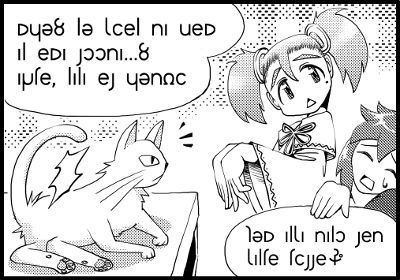
\includegraphics[width=0.5\textwidth]{ARKA/uni3.png}%或者height=\textheight
\end{figure}


% \emoji{l_sena}
% 那个棕毛就是``大姐姐 Mifa''哦。

% 穿着和我一样的``laasa''呢.


% \emoji{a_sena}
% 那个``laasa'' 是Lein穿的斗篷.


% \emoji{l_sena}
% Mifa 脾气短,因为 Xia 总是恶作剧,她就止不住地发飙.

% 不过仍然对Xia很好.

% \FiveStar 转写

% miifa: myu? lu xiel na vem al ema soona...? arte, lala es yundi


% \emoji{x_asex}
% ``myu'' 在第一格已经学过了.

% ``lu xiel na vem al ema soona...?''哦?
% 。最后的soona属于sete座椅还是疑问句呢.

% lu在\hyperlink{chapter-pronouns}{代词}这一章已经学过了,确认一下,是``他/她''.

% 额,猫不用tu(这),而是用lu(他)么?


% \emoji{a_sm}

% 毫无问题.因为和人类比较近,所以用lu.


% \emoji{x_loki}
% 是这啊.后面的xiel是什么?动词吗?

% ----

% xiel

% [游离副词][形容词]恐怕、万一、说不定、一旦

% 19:恣意

% [语法]

% aluut

% ----

% \emoji{l_asex_kal}
% 说是游离副词呢.语法就参考Aluut.

% aluut就又说来话长了,我来总结一下:

% ``恐怕'',``绝对''之类``表示概率的单词'',放在动词的前面.

% ``总是'',``偶尔''之类``表示频率的单词''也一样.


% \emoji{x_pil}
% %    <a href=``study_mive1_9.html''
% 表示\hyperlink{chapter-imperative}{命令}的re一样,是放在动词的前面呢.在语法上是re和en的同义词.

% na是什么意思啊.既然xiel放在动词前面,这就应该是动词吧.

% 意思好像是``感到''.

% ----

% na     

% [名词]心  

% [动词]感觉,感到 yul.   

% [文末纯词]像~一样。推断``总觉得是那样''  


% ----

% \emoji{x_demo}
% 是``感觉''啊.vem,vem,vem......妖ー怪ー、人ー类ー (略

% 啊啦、vem是``可怕''的意思呢.好巧啊.


% \emoji{l_hik}

% (紫苑、妖怪是bem啊......\footnote{原文为``妖怪人間'',指外貌像人类的妖怪})


% \emoji{x_asex}
% a non是``对我'',这里指的是被吓到的对象吧.

% 也就是说,``lu xiel na vem al ema soona...?''就是``也许他吓到我了''么.

% 哈哈哈.确实,你看洋洋的表情,和第一,二格不一样呢.确实是吓着了.

% 所以Mifa说的是``那个,那孩子很可怕么?''.



% \emoji{a_rans}
% 后面的arte跟英語的``Oh my god!''差不多.``哎呀''之类的。

% lala是表示惊讶的开头吧。


% \emoji{x_lo}
% es意思跟``怎么''差不多.

% yundi是eyo吗。

% ----

% eyo

% [文末纯词][milia]~是么

% 古:eyo。始于lydia的句末纯词.

% [语法]

% 表示对句子真实性不确定的模态.

% ----

% \emoji{x_loki}

% eyo是``~吗''。

% 所以是``啊啦,怎么了''的意思么. 

% 被猫吓到了才这么说么.

% 好了,到下一个对话框吧.


% \emoji{a_niit}
% 返回去太麻烦了,我归你再放一遍吧.


% \begin{figure}[H]
% 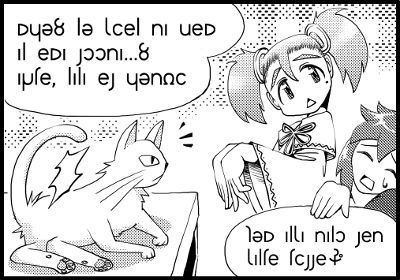
\includegraphics[width=0.5\textwidth]{ARKA/uni3.png}%或者height=\textheight
% \end{figure}

% \emoji{l_niit}
% 右下是Xia的吐槽哦。

% 最后的记号叫axte,像是日语的(笑).
% \footnote{补充一下,日语的``草'',由``wwwwwwww''象形而来.由于``笑''是``笑う(wa ra u)'',弹幕中常用``wwwwwww''代表``爆笑''.
% 后来有``草(中日双语)''之类的梗.英语版此处用的是`` :) ''.
% }

% \FiveStar 转写

% xia: kum alxa nalo sen xalte tisse (axte


% \emoji{x_pil}
% kum......是动物啊。

% Lein,我还是不明白alxa.

% ----

% alxa 

% [形容词] 所谓的~ 

% 古:alxa(所有的)。与 ``xaxa(存在/存在)''同語源。但是alxa和xaxa意味不同.

% [语法] 

% 用于名词,只带这个名词对应的所有个体.min alxa意思是``凡是女人'',表示所有的女人。
% 理论上和 ``il min'' 相同,但是il min和``every''差不多,注重个体的成员.

% [用例]

% vik alxa et ibet a vort. 男人都是幼稚的东西。

% ----

% \emoji{l_asex_kal}
% 译作 ``凡是~'',用于一般化的指代全体。

% kum alxa意思是``所有的动物''、min alxa是``凡是女的''.


% \emoji{x_sena}
% 哦哦 ♪

% sen在\hyperlink{chapter-adverb}{副词}讲过了,是``能''nalo sen是``能察觉到''。
% %senは<a href=``study_mive1_6.html''
% xalte是目的语,意思是``氛围''.所以,意思是``能察觉氛围''.


% 啊,简而言之就是“会读空气”吧?


% \emoji{l_sena}
% 对了哦.


% 最后的tisse和sete一样是文末纯词,做给对方透露情报的时候用.

% 像是``~だよ''.


% \emoji{x_nal}
% 顺便,``kum alxa nalo sen xalte tisse (axte''意思是``动物也会读空气啊(笑''。

% 哈---哈---``Mifa这么能发火,但还是害怕猫呢'',Xia吐槽的是这个.

% 嗯,才学了这么多,我就连Arka的吐槽都能看懂了......(\^{}-\^{};

% 词典真厉害啊。不用记也能看。

% 啊,终于到最后了!
\begin{figure}[H]
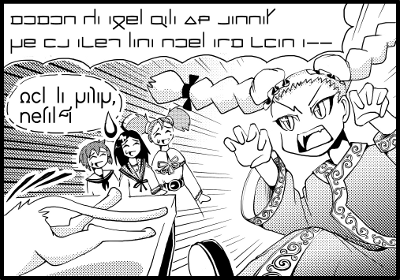
\includegraphics[width=0.5\textwidth]{ARKA/uni4.png}%或者height=\textheight
\end{figure}


\emoji{l_reia}
那个金毛丸子头就是``孩子气的Feel''哦。穿着叫做``teebe''的长袍。


\emoji{a_sm}
teebe也是Arna大学的制服,

テーベもアルナ大の制服で、像我这样的Raudura学院的学生经常穿。

普通科这么穿到时很少见……。


\emoji{l_nakx}
Feel虽说也是Arna的人,但就是有点怪。

她觉得自己是从神话时代转生过来的
\footnote{她以为自己是Kmiiir的转世.Kmiir则是Axet的一员,从恶魔手中拯救世界.}
。所以和占卜师Aria穿的是同样的teebe。

长得娇小(矮),所以有些烦恼、活泼得很,说话总是能这样那样地离题。

很会搞事情,但这样才有趣嘛。


\emoji{x_iks}
2333w  看那个脸 w

就像要把猫抓来吃了一样呢w

好像文字的设计也在这里变化了呢。好细啊。


\emoji{a_reps}
看,转写

\FiveStar 转写

feel: momon ca adel fala 85 sanna! re is axek lana noel atm xian a--


\emoji{x_demo}
额,首先momon是个啥。
    
\emoji{x_seernik}
……蛤?  [魔物]……?  啥啊。

----

momon

[魔物]momon(猫熊):第八十五天:利之空天

19:ridia/seren/mel : 源自叫声

[文化]

妖族。矮胖而像猫和熊。体型像大些的兔子。
它们有一个惹人爱的习惯,就是变化成人们饲养的宠物。会发出``momon''的奇怪声音。对主人忠实,很驯服。

----

\emoji{l_xanxa}
我快把这忘了,Arbazard还是异世界呢(-_-; 也就是``剑与魔法的幻想''。

在我的时代已经绝迹了,曾经有100种魔物呢。

说``八十五天''是指momon是怪物里的第85号。

momon是很珍贵的魔物,不会伤害人类.就像宠物一样。

\emoji{l_ket}
我也想养一只momon啊。

为啥不来我家捏\~{}。


\emoji{x_nal}
モ○グリ啊,明白了。


\emoji{l_iks}
额……。


\emoji{x_niit}
ca是表示强调的形容词、像英语的the一样。

momon ca adel 就是``mmon・the・monsterー\Fivestar''这样的感觉吧?

----

ca

[形容词]这。增加强调和限制意味,前置使用。

[形容词]表示后面的是固有名词。前置使用。

[名词]``*''号

17:制:古:ca(表示强调的形容词,有冠词性)

【用例】

varfant, ca freian 剑士Varfrant

----

\emoji{l_diina}

对,在同一格。","记号叫做``tsunk''、写不写都可以。

fala 85在上面也有提到、意思是85号的魔族。fala是表示序号的格词。


\emoji{x_loki}
sanna是表示确认的,总体来看``momon ca adel fala 85 sanna!''就是``你就是第八十五天的momon吧!''的意思呢。

哈啊,搁着Feel把猫当成魔物了。

确实、离谱的神話志向妹 (-ω-;

\begin{figure}[H]
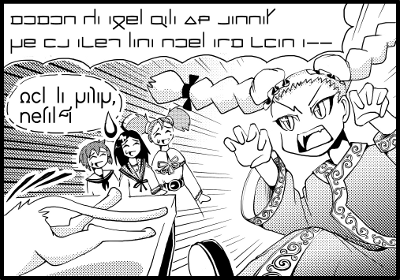
\includegraphics[width=0.5\textwidth]{ARKA/uni4.png}%或者height=\textheight
\end{figure}


\emoji{x_asex}
接下来是``re is axek lana noel atm xian a...''这句。

re在``命令・依頼・禁止''学过了,表示命令。

is是死生动词那一课的``死动词'',``关闭,停止''.


\emoji{l_deyu}
动词is的宾语是axek(変身)。

尽管日语的``変身を解く(解除变身)''里面要用``解く(解除)''作动词搭配、,Arka里直接写is就行了。

\emoji{x_niit}
因为宾语axek已经明确了,后面就不再带名词。

lana既有名词又有格词的用法、但这里确定是格词。表示``为了做''。

noel是我(私)、xian是你――指猫。

atm……``卖''。额、卖猫?


\emoji{l_reiv}
好像是  (-_-;

haizen(报应啊)


\emoji{x_knoos}
最后的a是啥……。

唉、哎哎哎、a是什么意思啊!?


\emoji{a_sm}
在句末的话、应该是a(4)。只是整理语气,没有特别的意味。

----

a(4)

[文末纯词]"\~{}吗","\~{}嘛"\footnote{~だな、~か}。短的感叹。

古

[语法]

a系列用于自身。e系列用于听者。a系列对他人使用是男性的语气。
对于长辈和上级则失礼。即使是同级,如果不是非常要好,也会令人觉得草率。

----

\emoji{l_nax}
顺便一说,对他人说话还是用e比较合适。

只是,a还有额外的格词用法``为了~''。意思是``为了卖~''。

----

a

[格词]为~、为了~。与格。

[格词]向~对应的神祈祷时、不能用a,而应当用al。al karte就是沿袭古代祷词的用法.

13:制:al。为了区别于新的接续词al而改短了。

[语法]

动元音开头的单词用al。比如al an(向我)。

关系从句中只有格词残存的时候也用al。tu et ridia l'an fitat miik al(我给苹果的人是ridia)

【用例】

fit a lu. 给他。

fit al an. 给我。

----

\emoji{x_fron}
额……可是、a后面啥都没有了?卖的对象呢。


\emoji{l_niit}
这句话在这就截止了。

卖给谁就不清楚了、本来这里应该是买家的。

日语里台词的中间就有「(略」或者「(ry」的写法呢、只是不常用.


\emoji{x_loki}
あぁ、「(略」のことね。それで格詞のaだけ残ってるのか。
じゃあまとめると、"re is axek lana noel atm xian a..."は「私があなたを売るために、変身を解きなさい!」ってことか。
ふぇーるは猫を魔物が変身したものだと思い込んでるようね。困った子だわ(;´∀`)
ところでアリア、左上に3人が並んでいるけど、これは……?。

<a href="uni4.png" tppabs="http://conlinguistics.org/arka/images/uni4.png">
<img src="uni4.png" tppabs="http://conlinguistics.org/arka/images/uni4.png" target="_blank" hspace="15">
</a>


\emoji{a_lo}
3人とも「ふぇーる」の言動を見てドン引きしてるみたいね。
最後の文字はアリスといって、不安などを表すの。転写するときはalisでいいわ。

☆転写
dil la rakar, netal (alis


\emoji{x_knoos}
dilは「邪魔をする」という動詞みたいだけど、いきなり動詞が来るの?
アルカは「主語+動詞+目的語」じゃなかったっけ?


\emoji{a_sm}
命令文では主語を省略できるのよ。


\emoji{x_nakx}
あ、そうか。そういえば前にやったね。
dil laで「彼女を邪魔しろ」……つまり、「彼女を止めろ」という意味かな。
あれ、でもrakarは「狂信者」という名詞のようね。laとrakarで名詞が連続しているよ。ヘンじゃない?

----

la
    [代詞]彼、彼女、あの。前置。
[反意語]lu
13:恣意
【用例】
la fian あの少女

----

\emoji{l_xanxa}
うん、これはちょっと難しいから、順を追って話すね。
代名詞は正確には代詞というの。どうして代詞というんだと思う?


\emoji{x_demo}
えぇと……。分かりやすさを考えれば、本来は代名詞と命名するはずだよね。
わざわざ「名」を抜くからには、名詞以外の使い方もあるってことじゃない?
例えば、代……動詞とか、代……形容詞とか。わかんないけど。


\emoji{l_ket}
さすが紫苑!そうなの。形容詞や動詞としても使えるから、代名詞じゃなくて代詞と呼んでいるのよ。
辞書をよく見ると、「彼」のほかにも「あの」と書いてあるね。
la rakarは「彼、狂信者」ではなく、「あの狂信者」という意味です。


\emoji{x_sena}
なるほどね!
「前置」と書いてあるとおり、形容詞用法のlaは名詞の前に置くのね。
ふつうアルカの形容詞は名詞の後ろに来るから、laは特殊なんだね。


\emoji{l_deyu}
この使い方はtu(これ), le(あれ), lu(この)にも言えるの。
tu miikで「このリンゴ」、le galtで「あの門」、lu fianで「この女の子」になるよ。
生きてるものにはluやlaを使ってね。


\emoji{x_knoos}
ねぇ、ここではla rakarになってるけど、どうしてlaなの?
luじゃダメなの?


\emoji{a_rans}
lu rakarでも文法的には正しいわ。
でもここではlaのほうがいいの。どうしてだろうね。
紫苑、luとlaの違いはなんだっけ?


\emoji{x_niit}
えっと……確か距離だよね。luが近くて、laが遠い。


\emoji{a_sm}
その距離っていうのは、心理的な距離も指すのよ。
みんなここでは「ふぇーる」に対して「ドン引き」してるでしょ。
引いた分、心理的な距離が遠ざかっているから、それがla rakarという表現に現れてるのよ。


\emoji{x_tisse}
なるほどぉ!よく分かりました。
えと、最後のnetalは「誰であろうと」という意味みたいね。「誰でもいいから」とか「誰かしら」という意味かな。
ってことは、"dil la rakar, netal (alis"は「誰かあの狂信者を止めろ(汗」になるのね。
ねぇ、どうして狂信者って単語が出てきたの?


\emoji{l_reia}
私の時代には魔物がもういないからね。
猫が魔族モモンだって疑うのは、よっぽど神話に心酔しきった人なのよ。


\emoji{x_sena}
あは、そういうことね☆
ようやくオチの意味が分かったよ。
それにしても、たった1つの4コマで、かなりのことが学べるんだねぇ。驚いたよ。


\emoji{l_sena}
言語はもちろん、文化背景まで分かるようになるからね。
紫苑も最初の頃に比べたら、ずいぶん辞書を引くのが早くなったね。
マンガは良い教材になると思うよ。「ねこにっき」の続きも紹介しておくね→<a href="works_xale_1.html" tppabs="http://conlinguistics.org/arka/works_xale_1.html">ねこにっき</a>


\emoji{x_pil}

全部で21話もあるんだ!?うはぁ、ここでやったことがあと20個も!これは勉強になるわ。
代名詞はnonとかnoelとか色々あるけど、読んでるうちに慣れちゃいそう。


\emoji{l_rana}
さて、今回の練習で、画面の前のみなさんも、幻日辞典の使い方が身に付いたと思います。
紫苑と私が読み進めていったやり方で読んでいけば、どんな文でも読めるようになると思いますので、ぜひ辞書を活用していってくださいね☆ミ


\emoji{x_nal}
「はじアル2」就到此为止了、谢谢观赏!
各位读者也辛苦了!


\emoji{l_nax}
感谢您长时间的支持!

紫苑和ridia也辛苦了。我烤了戚风蛋糕、关掉电脑等一会啊。


\emoji{x_flip}
哇------♪</p>



